\documentclass[11pt, oneside]{article}
\usepackage{geometry}
\geometry{letterpaper}
\usepackage{graphicx}
\usepackage{amssymb}
\usepackage{amsmath}
\usepackage{tikz}
\usepackage{tikz-qtree}
\usepackage{url}
\usepackage[T1]{fontenc}

\title{SICP Exercise 3.16}
\author{Yuchong Pan}

\begin{document}
\maketitle

The box-and-pointer diagrams representing list structures made up of exactly three pairs for which Ben's procedure would return 3, return 4, return 7, and never return at all are given as follows, respectively.

\begin{figure}[h!]
    \centering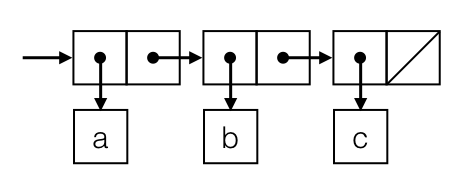
\includegraphics[width=7cm]{ex-3.16-1.png}
    \caption{List structure made up of exactly three pairs for which Ben's procedure would return 3.}
\end{figure}

\begin{figure}[h!]
    \centering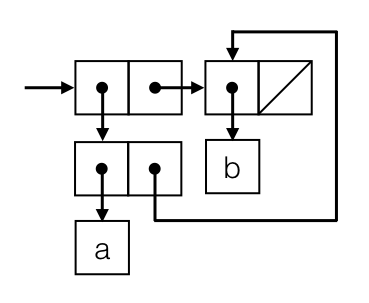
\includegraphics[width=7cm]{ex-3.16-2.png}
    \caption{List structure made up of exactly three pairs for which Ben's procedure would return 4.}
\end{figure}

\begin{figure}[h!]
    \centering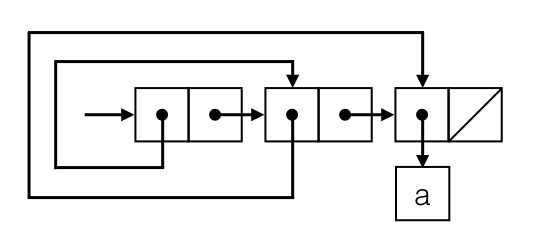
\includegraphics[width=7cm]{ex-3.16-3.png}
    \caption{List structure made up of exactly three pairs for which Ben's procedure would return 7.}
\end{figure}

\begin{figure}[h!]
    \centering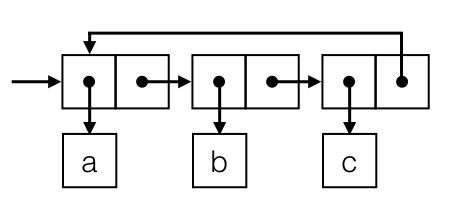
\includegraphics[width=7cm]{ex-3.16-4.png}
    \caption{List structure made up of exactly three pairs for which Ben's procedure would never return at all.}
\end{figure}

\end{document}
